\chapter{Chrétiens et musulmans au XIX et XXe siècle}

\mn{11/04/23 Charbel Attalah}

\section{Historique}

\paragraph{Révolution industrielle}
Extension coloniale grâce aux nouvelles techniques.


\paragraph{1798 - 1801 Egypte} pour gêner la puissance coloniale de l'Angleterre.

Cela aura comme l'une des conséquence 

\paragraph{1830 - Algérie}

\paragraph{1857 - Inde rattaché directement à l'Etat Anglais}


\paragraph{Empire Ottoman au plus bas}

Non empéché par la Grande porte : 
\begin{itemize}
    \item Première rencontre : Abdel Kader va empécher le massacre des libanais en 1860. Vague d'exil des chrétiens d'orient au Brésil (13 millions de libanais en diaspora).
    \item 1895 extermination des Arméniens et Kurdes
\end{itemize}

\begin{Synthesis}
Quelle réaction ? 
\end{Synthesis}


\section{Quelques noms du Controverses du XIX }

\subsection{Missions chrétiennes}

\paragraph{prédications protestantes}

\paragraph{William Muir (1819-1905)}
Son frère s'intéresse à l'hindouisme. Son frère William va s'intéresser aux études islamologues
\begin{itemize}
    \item 
    \item le témoignage du Coran en faveur du Christianisme
\end{itemize}
Conversion personnelle quand il décide de vivre avec des musulmans.


\paragraph{Karl Pfander (1803-1860)} \href{https://en.wikipedia.org/wiki/Karl_Gottlieb_Pfander}{Pfander} va déterminer 
Il était persuadé que la controverse pouvait faire tomber un pays musulman.
Il va nous laisser un livre, la \textit{balance de la Vérité}, \textit{Mizan al-Haqq} très large. 

3 parties : 
\begin{itemize}
    \item L'authenticité des écritures \mn{On n'est plus sur la trinité}. Falsification des écritures et authenticité de la bible. Démontrer que la Bible n'est pas abrogée. 
    
    \item l'enseignement fondamentale de la Bible
    \item prétention de l'Islam à être la Révélation finale. S'attaque à Mohammed
\end{itemize}

Va être très mal reçu

\subsection{réactions de l'Inde}

\paragraph{Rahmatullah al-Kauramawi (1818-1891)}  Va répondre par un livre \textit{Izhar all-Haqq}, la \textit{manifestion de la vérité}. 

\begin{Prop}
Besoin de la rencontre : sinon, on reste dans la polémique. 
\end{Prop}


\paragraph{Commentaires musulmans des livres de la Genèse} Intéressant. 

%---------------------------------------
\section{Réformistes Egyptiens}


\paragraph{Mohammed Abduh} L'islam est plus moderne que la modernité elle-même. Mais il faut revenir à l'Islam lui-même. Idée que toute la science se trouve dans le Coran.

Face à l'attaque moderne, l'Islam est la religion de la raison et le christianisme est une religion irrationelle.

\textit{tafsir Al-Manar} Son livre le plus célèbre. Il édite le périodique \textit{Manar}.
Face au Christianisme, publie une collection d'articles sur le christianisme essentiellement irrationnel. Une religion fuyant le monde, va condamner Galilée.


Devient le cheikh d'Al Azhar.

\paragraph{Risalat al Tawhid} L'enfance, c'est Moise (on a besoin de loi), le christianisme est adolescent, sentimentalisme, et l'âge adulte, c'est l'Islam. Cette force va avoir une grande influence. 

\paragraph{Une idéalisation de la science} Ambivalence, à la fois idéalisée et à la fois redoutée par rapport à son origine occidentale. Montrer que la science islamique. 
\begin{quote}
    si on avait respecté l'Islam, par rapport à l'[écologie], on ne serait pas là.
\end{quote}

\paragraph{Rashid Rida (1865-1935)} son disciple. Forme moderne des arguments médiévaux. Va essayer le \textit{pan-islamique}. Il a  vécu la fin de l'empire ottoman et vit mal l'arrivée d'Ataturk.
Pour ré-islamiser le monde, il va former un séminaire missionnaire musulman (1909).

\paragraph{Rida et l'Evangile de Barnabé} Ecrit au XVIIè, traité apologétique des morisques. Ceux qui ont fuit en Turquie et Tunisie ont pris leur revanche avec l'écriture de cet évangile \textit{Ibrahim al Tagbili - Juan Perez}. \textit{Christianisme, inventé par Paul}.  Pharisiens : ce sont les inquisiteurs. 

Mais pose problème pour les musulmans : 
\begin{itemize}
    \item Marie accouche sans douleur (alors que Co 19, 23)
    \item il nie que Jésus est le messie (alors que le Co l'annonce)
    \item Il est décrit comme prophète du monde entier (ce que lui réfute le coran)
\end{itemize}
Rida revient sur ce texte.  Avec les réformistes, il y a un débat sur le statut des écritures, mais sur Jésus lui-même. Attaque ad hominem, de part et d'autre.  

\paragraph{Frères musulmans coupent avec Rida et Abduh} A la fin de sa vie, Rida se coupe avec Afghani et Adbuh et annonce les frères musulmans. 
\paragraph{Y a-t-il  rupture  ou  continuité  entre  l’islam  politique  et  le mouvement du réformisme musulman?} Plusieurs islamologues arabes et  occidentaux  voient  dans  l’islam  politique  un  prolongement  du réformisme  musulman.  L’égyptien  Mohammad  ‘Amâra,  par  exemple, pense que le courant musulman \textit{« de résurrection et de renouveau »} de Jamâl  al-Dîn  al-Afghâni  et  Mohammad  ‘Abduh  se  poursuit  dans l’école  du  Manâr,  dirigée  par  Cheikh  Mohammad  Rachîd  Ridâ,  pour aboutir  à  l’association  des  Frères  musulmans,  fondée  par  Hassan  al-Bannâ,  et  celle-ci  est,  pour  lui,  la  première  organisation  de  masse  à exprimer  les  idées  du  courant  musulman  « de  résurrection  et  de renouveau» [‘Amâra, 1995, p.  18]. Nous  faisons  l’hypothèse  contraire,  à  savoir  que  l’islam  politique, incarné par l’association des Frères musulmans et les mouvements qui en  dérivent,  \textit{a  rompu  avec  le  réformisme  musulman  d’al-Afghâni  et‘Abduh }; 

selon nous, le Cheikh Mohammad Rachîd Ridâ, en répudiant à  la  fin  de  sa  vie  les  idées  de  ses  maîtres,  a  préparé  cette  rupture, détruisant ainsi tous les espoirs de changement que portait ce courant majeur de la pensée de la \textbf{Nahda}(Renaissance) qu’était le réformisme,et provoquant la régression des Lumières dans la pensée arabe
\mn{2006 le choc colonial et l'Islam \textit{Maher Charif} \href{https://www-cairn-info.icp.idm.oclc.org/feuilleter.php?ID_ARTICLE=DEC_LUIZA_2006_01_0517}{Réformisme musulman et islam politique : continuité ou rupture ?}}

\section{Problème des missions musulmanes}

\paragraph{Zèle ismaelien}

\paragraph{Equivalence de missions} pas de traduction de \textit{Evangélisation}. \textit{Da'wa} est utilisé pour \textit{Evangélisation} et \textit{prosélytisme}. Darwa veut dire \textit{invitation} mais vu aujourd'hui dans un sens négatif de prosélytisme. 

\paragraph{Al Armaddya} pas soufi, musulmans très orthodoxes. Rapport maître et disciple. Le maître est ici important. ils croient que Jésus a bien été crucifié mais descendu de la croix, toujours vivant et qu'il vit en Inde. 

\paragraph{Al Azhar} L'université de Fez au Maroc, Zitouna à Cordoue et \href{http://www.azhar.edu.eg/Graduate-Studies}{Al-Azhar} au Caire (8ème). Une partie de la faculté est consacrée à Da'wa. 

\paragraph{La ligue du monde Islamique} Dans le premier texte, protéger les chrétiens et après les convertir. Cette ambivalence se retrouve au sein d'une même institution mais elle nous habite tous. 


\paragraph{Formation des prêtres du 93} Toutes les tendances chrétiennes actuelles.

\chapter{Conclusion}

\mn{18/4 Marie Carmen et Charbel}

\section{bibliographie}
\begin{itemize}
    \item catalogue de l'exposition \textit{coexistences}
\end{itemize}
\section{rappel du plan}
\begin{itemize}
    \item Braudel
    \item espace fragmenté
    \item Louis Gardet, Massignon, et xxx : des passeurs.
\end{itemize}

\section{cosmopolitisme méditerranéen}

\begin{Synthesis}
    idée que le cosmopolitisme est d'abord méditerranéen et copié ensuite ?
\end{Synthesis}

\begin{Def}[ville cosmopolite]
plusieurs définitions possibles :
\begin{enumerate}
     \item plusieurs religions dans un même endroit et cela marche(rait)  
    \item il faut rajouter communauté d'intérêt (Robert Ilbert). Avant même d'être dans l'empire ottoman, on est d'abord Stambouliote, ...
  \item rattaché non seulement à la ville mais à plein d'espace (une plante cosmopolite)
\end{enumerate}
 \end{Def}

\paragraph{l'âge d'or cosmopolite au XIX} des communautés avec minet et colonie et \textit{cela fonctionne}. Mariages mixtes,... \mn{Roman de L. Durrell, le \textit{quatuor d'Alexandrie}}

\paragraph{importance du regard et de l'approche} si on regarde les documents accessibles (procès,...), on a plutôt une vision négative. Il faut regarder dans le détail des relations.

\paragraph{deuxième âge : Mort par la poussée nationaliste} Mort des villes cosmopolites à des dates différents : 
\begin{itemize}
    \item Salonique (1912)
    \item Alexandrie (1958)
    \item Beyrouth (denière ville cosmopolite)
\end{itemize}
Les gens avaient des identités plurielles et on leur demande de fixer leurs identités (si "Français", alors 'vous devez vous battre'). 

Des barrières de plus en marquées. Alexandrie pert sa proéminence par rapport au Caire. 


\paragraph{troisième âge : nouveaux cosmopolites} Suite à la mondialisation. Vraie question : est ce qu'on parle de la même chose d'avant ? Au lieu de parler de coexistence, on va parler de \textit{co-présence} ? On vit à côté de l'autre.
Un géographe qui a étudié Beyrouth a parlé de co-présence : cette façon de vie à côté de l'autre et non \textit{avec l'autre}.
\begin{Ex}
A la sortie de la messe, est ce qu'on vit quelque chose ensemble ou est-ce qu'on vit dans l'entre-soi ? 
\end{Ex}

\paragraph{Exposition Coexistence} D. Albera et M. Penicaud.  Exemples de lieux de coexistence, y compris théologique.
\begin{Ex}
    Monastère Saint George à Istamboul, qui est aujourd'hui un lieu de pélerinage pour les musulmans.
    \textit{Depuis l'arrivée sur l’île, il faut compter 20 minutes de marche pour aller jusqu'au sommet. Si vous visitez les environs autour du 23 avril (la Saint Georges), vous remarquerez sur votre chemin des fils de couture (symbolisant les vœux) suspendus aux arbres et aux broussailles. Les Turcs musulmans et les orthodoxes célèbrent cette fête. Une fois au sommet, profitez de la vue magnifique. Vous y trouverez un restaurent prêt à vous accueillir pour un rafraîchissement.}

    \begin{figure}
        \centering
                \sidecaption{Monastère de Saint-Georges, Istanbul. Visiteuses bloquées dans les fils votifs.
 (Manoël Pénicaud)}
        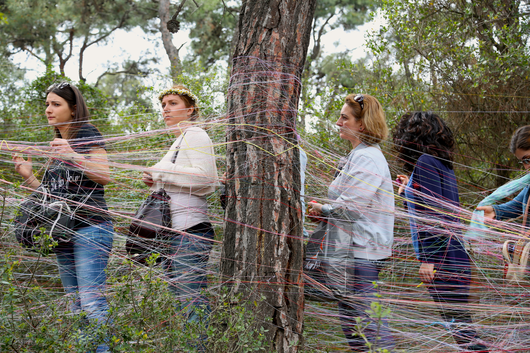
\includegraphics[width=\textwidth]{HistoireIslamMediterranee/Images/StGeorges.png}
 
        \label{fig:my_label}
    \end{figure}
\end{Ex}

Il faut faire la différence entre lieu saint et lieu de culte. Les lieux saints sont plutôt chargés de quête spirituelle et plus des lieux d'échange.

Ils veulent se démarquer des courants passés :
\begin{itemize}
    \item impossibilité des contacts qui cherchent d'abord les conflits
    \item un autre mouvement, où il n'y a  plus de peur entre les deux
\end{itemize}
Eux se positionnent entre les deux. 

\paragraph{Les figures de Saint Georges, Marie} figures consensuelles

\begin{Ex}[Cathédrale d'Alger ]
     \textit{priez pour eux et pour les musulmans}. Abd El Kader. 
     \begin{figure}
         \centering
         \includegraphics{}
         \caption{Caption}
         \label{fig:my_label}
     \end{figure}\href{https://fr.wikipedia.org/wiki/Basilique_Notre-Dame-d%27Afrique}{Notre Dame d'Afrique}
\end{Ex}

\begin{Ex}[Apparition de la vierge au Caire en 1968]
    Al -Kodr
    trois musulmans qui ont une apparition de la Vierge au dessus d'une Eglise copte.
    \href{https://fr.wikipedia.org/wiki/Notre-Dame_de_Zeitoun#:~:text=Notre%2DDame%20de%20Zeitoun%20est,Caire%2C%20de%201968%20%C3%A0%201971.}{Apparition}
    Contexte de la guerre des 6 jours, qui est vu comme une catastrophe en Egypte.

    Avec le développement de l'Islam rigoriste, ce pèlerinage s'arrête.
\end{Ex}

\paragraph{Chant Ave Maria et Allah Akbah}

\paragraph{ne pas gommer la différence} On risque de tomber dans le syncrétisme. Bien que le militantisme et les controverses continuent, on est dans une nouvelle approche.

\paragraph{la symétrie n'est pas chrétienne} L'action de Dieu est toujours asymétrique. 

\paragraph{privilégier les relations} l'incarnation. 

\paragraph{La théologie byzantine} probablement une théologie désincarnée. C'est celui qu'a rencontré l'islam ? La majorité des controverses sont théologiques. 